%==WORKHEET 1
\newpage
\stepcounter{handout}
\begin{exercisebox}[adjusted title=First Program]
Type the following example in the Processing editor and press

\includegraphics[height=4mm]{illustrationer/processing_play_button}-button:

\begin{lstlisting}[language=JavaScript]
function setup() {
  //set the canvas and background color
  createCanvas(400, 400);
  background(220);
  
  // Tree
  rect(55, 50, 10, 20);
  ellipse(60, 35, 30, 40);
}

function draw() {}


\end{lstlisting}


Then add the following into the setup() function:
\begin{lstlisting}[language=JavaScript]
  // powerplant
  rect(120, 50, 60, 30);
  rect(160, 20, 10, 30);
  triangle(120, 50, 136, 40, 136, 50);
  triangle(136, 50, 152, 40, 152, 50);

\end{lstlisting}
And:
% \begin{python}
% # Person
% ellipse(270, 65, 8, 8)
% line(270, 70, 270, 75)
% line(270, 69, 277, 75)
% line(270, 69, 263, 75)
% line(270, 75, 275, 82)
% line(270, 75, 265, 82)
% \end{python}
\begin{lstlisting}[language=JavaScript]
  // windmill
  line(300, 50, 320, 51);
  line(300, 50, 289, 67);
  line(300, 50, 291, 32);
  line(300, 50, 300, 90);
\end{lstlisting}

\tcbsubtitle{Now try drawing a car and a cloud:}
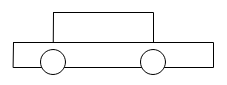
\includegraphics[width=0.4\textwidth]{illustrationer/bil-streg.png}
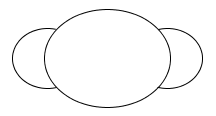
\includegraphics[width=0.3\textwidth]{illustrationer/sky.png}
\end{exercisebox}

\begin{exercisebox}[adjusted title=Colors]
You are now going to colour the shapes. To do this, use the
\ttpy{fill(r, g, b)} function, which selects which colour 
to use for fill and text colour. It's all about calling
\ttpy{fill} in the right places! As arguments, you specify the amount
of red (0-255), blue (0-255), and green (0-255).
\noindent
Here are some basic colors to experiment with:
\begin{minipage}{0.45\linewidth}
\begin{lstlisting}[language=JavaScript]
fill(255, 0, 0);  // red
fill(0, 255, 0);  // green
fill(0, 0, 255);  // blue
\end{lstlisting}
\end{minipage}
\begin{minipage}{0.45\linewidth}
\begin{lstlisting}[language=JavaScript]
fill(0, 0, 0);       // black
fill(255, 255, 255); // white
fill(255, 255, 0);   // yellow
\end{lstlisting}
\end{minipage}

\noindent
Optionally, find colours using an online color picker or RGB
colour table. For example, search for ``RGB color picker''.
\tcbsubtitle{Lines and outlines}
To specify the colour of strokes (e.g. \ttpy{line}) and outlines, use \ttpy{stroke(r, g, b)}. Also try the \ttpy{noStroke()} function, to turn off outline drawing.
\end{exercisebox}

\begin{exercisebox}[adjusted title=Example]
\noindent
Here's an example of what it might look like after colouring:
\begin{center}
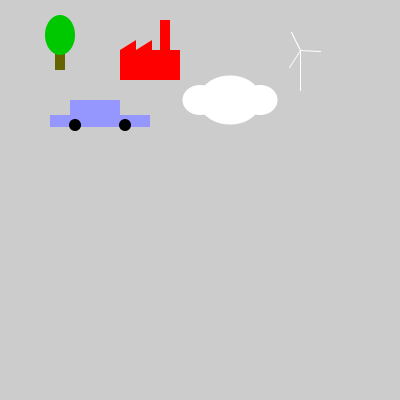
\includegraphics[width=0.5\textwidth]{illustrationer/farvelagt.png}
\end{center}
\end{exercisebox}

\begin{exercisebox}[adjusted title=Green City]
%Gem projektet og giv det navnet ``Elbil''. Senere skal vi udbygge dettil en simulation hvor bilen skal lades med strøm fra enten vindmølleeller kraftværket, men hvor bilen helst skal lades op med grøn strøm fra vindmøllen.

Use what you've learned to make it a slightly nicer scene, with background, foreground and the extra details you think should be there. For example, I've drawn a road and moved the characters around. 
\\
\\
\textbf{Tip: }To change the background color from gray you can use \ttpy{rect} which you
already know, but you can also use the \ttpy{background(r, g, b)} command.
It will delete everything and fill the screen with the specified colour.

\begin{center}
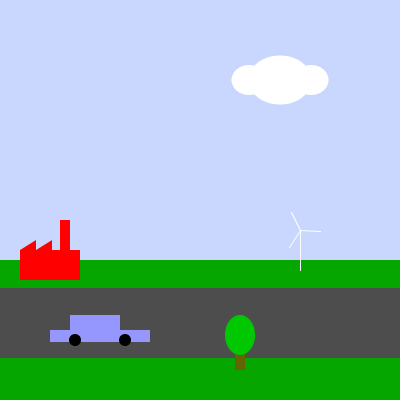
\includegraphics[width=0.5\textwidth]{illustrationer/elbil.png}
\end{center}

\noindent
Remember to use comments to find your way around the code easily!
Commenting code is good because it improves code readability and maintainability by explaining the purpose and functionality of the code to others and to your future self.



\end{exercisebox}
